% !TEX root = main.tex
\chapter{Wind Tunnel Experiment}
\label{chap:experiments}
  Verifying the simulated aerodynamic effects is imperative to verify the numerical analysis. In order to assess the reliability of the previously mentioned simulations, a physical measurement of the pressure along the down-scaled wing will provide results for comparison. When conducting tests on models, knowing how the flow behaves on different length scales and at different velocities is a requirement. Accordingly, this chapter starts with discussing the fluid theory behind the experimental setup.

  Measurements and tests have been carried out at the DTU Wind laboratory's Red wind tunnel with the help of our supervisor Robert Flemming Mikkelsen the 19\textsuperscript{th} to the 20\textsuperscript{th} of June.

\section{Aerodynamical Theory}

  The theories explaining how fluid effects scale between varying wing sizes is explained, in order to justify using a down-scaled model as evaluation to a real size wing.

  \subsection{Similarity of Flows}
  \label{sec:similarflows}

    In order to perform tests on the rear wing, it has to be scaled down to fit inside the wind tunnel. This reduces the physical size of the wing, which under equal circumstances changes the flow around it. In order to correctly emulate the simulated flow inside a wind tunnel, the Reynolds number of the full scale flow and the model scale flow has to be the same.
    \begin{align}
      \text{Re}_\text{m} &= \text{Re}\\
      \intertext{Mathematically, the Reynolds number are defined as:}
      \text{Re} &= \frac{u L}{\nu}
    \end{align}
    where $u_\infty$ is the velocity of the fluid in motion, $L$ is the characteristic length and $\nu$ is the kinematic viscosity of the fluid.

    For a down-scaled model, matching Reynolds number requires an increase in velocity, inversely proportional to the increase in length:
    \begin{align}
      \frac{u_\text{m} L_\text{m}}{\nu} &= \frac{u L}{\nu} \nonumber \\
      \Rightarrow u_\text{m} &= \frac{L}{L_\text{m}} u \label{eq:windtunnelspeed}
    \end{align}

    Given the nature of the competition, the average cornering speeds are around $\SI{55}{\kilo \meter \per \hour} = \SI{15.28}{\metre\per\second}$, which is where downforce is of most importance. The desired velocity in the wind tunnel for the scale model can be found from equation \ref{eq:windtunnelspeed}:
    \begin{align*}
      u_\text{m} &= \frac{\SI{0.6}{\metre}}{\SI{0.15}{\metre}} \SI{15.28}{\metre\per\second} = \SI{61.12}{\metre\per\second}
    \end{align*}

    Which in accordance to the range of the Red wind tunnel.

\section{Equipment}

  The equipment required for performing a wind tunnel test can be seen below:
  \begin{itemize}
    \item The Red wind tunnel ($\SIrange{60}{65}{\metre\per\second}$)
    \item 1/4 scale wing
    \item Syringe inserts for pressure taps
    \item Rubber tubing
    \item Strain gauge for lift
  \end{itemize}

  The instrumentation and the Red wind tunnel is described below, along with a thorough description of the scale wing designed and produced for the experiment.

  \subsection{Instrumentation}

    Instrumentation to perform the experiments were graciously provided to us by DTU Wind Energy. The following contains a description of the wind tunnel, datalogging devices and software used to perform the measurements.

    \textsc{The Red Wind Tunnel}

      The red wind tunnel is an open loop wind tunnel located at DTU Lyngby. A picture of the wind tunnel with our supervisor Robert Mikkelsen can be seen in figure \ref{fig:theredwindtunnel}. It measures $\SI{0.5}{\metre} \times \SI{0.5}{\metre} \times \SI{1.3}{\metre}$ in the test section, with a maximum wind speed of \SI{65}{\metre\per\second}. The wind tunnel functions in low Reynolds number, which fits with the chosen MSHD aerofoil.

      \begin{figure}
        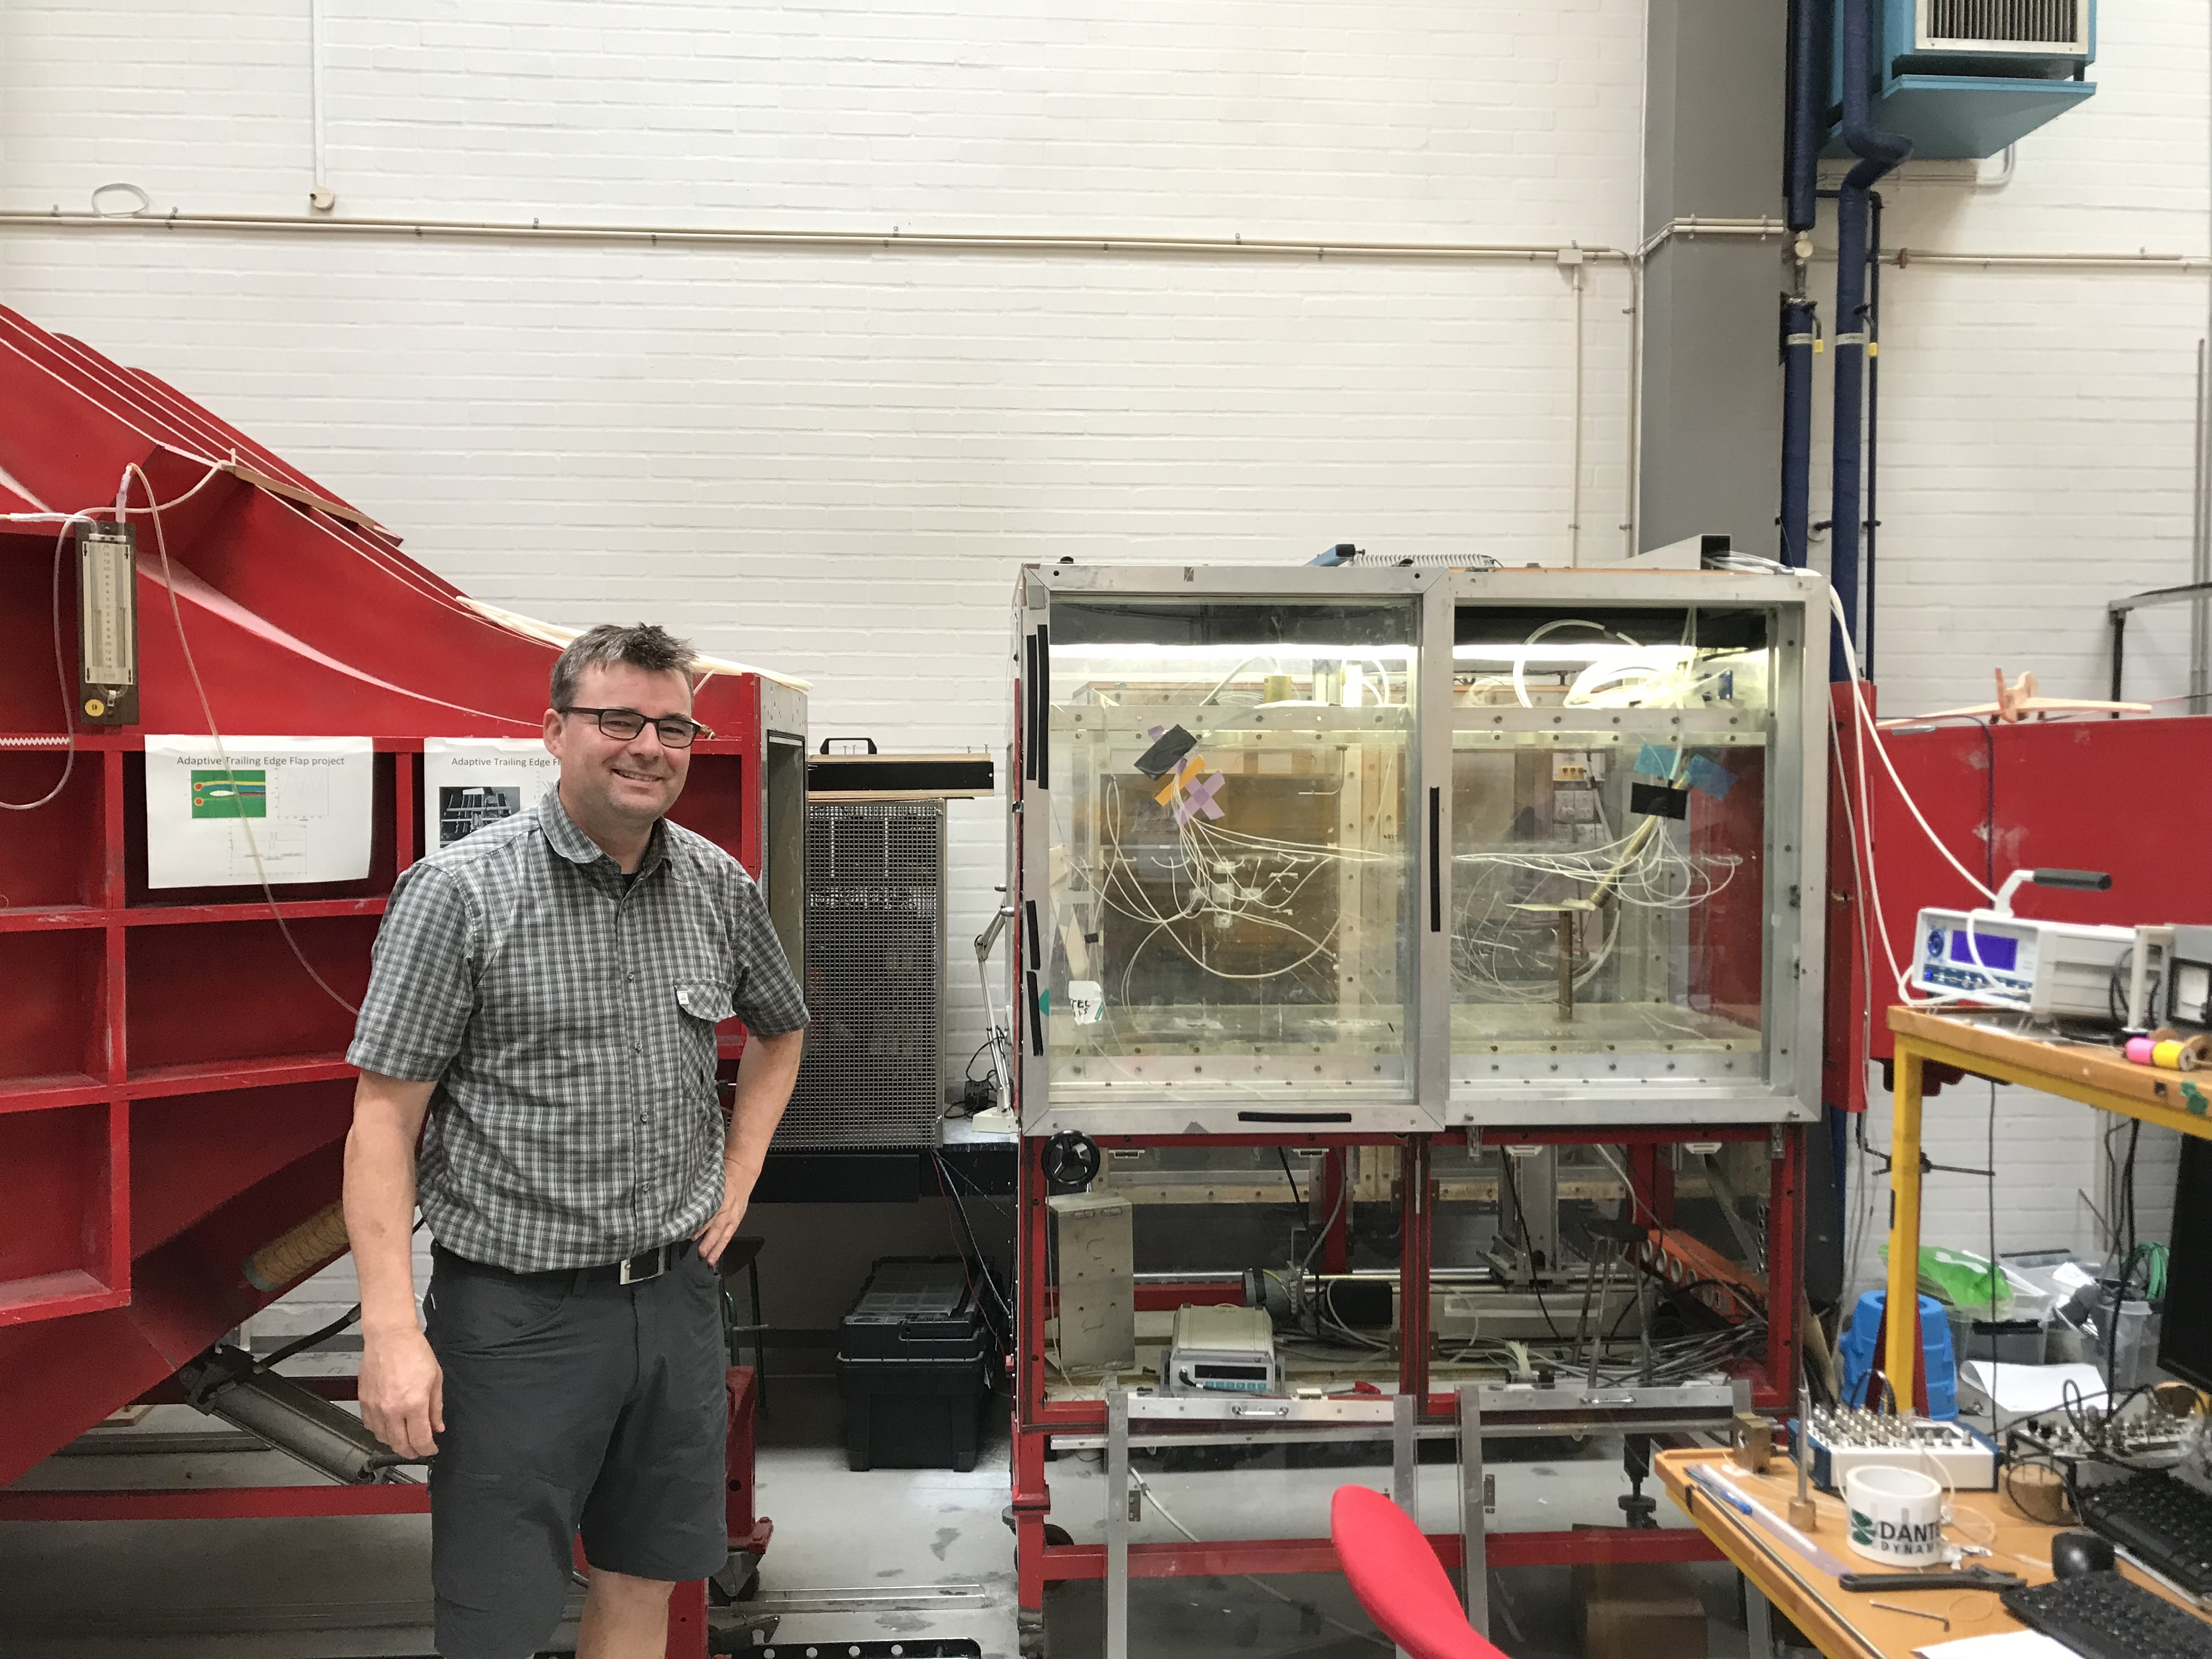
\includegraphics[width=\textwidth]{theredwindtunnel}
        \caption{Robert Mikkelsen posing in front of the Red wind tunnel. To the left is the air inlet, followed by the test section.}
        \label{fig:theredwindtunnel}
      \end{figure}

    \textsc{Pressure Measurements}

      The Red wind tunnel is equipped with data logging equipment measuring up to 64 pressure probes on a wing profile, the Angle of Attack (AOA), a force gauge measuring the lift forces, a pitot rake measuring the pressure in the wing's wake, the dynamic pressure in the wind tunnel, the operational speed of the wind tunnel, the air density and the time of measurement. The measurement equipment was connected to the data-logging software LabVIEW on a nearby computer.

  \subsection{Manufacturing the 1/4 Scale Rear Wing}

    When producing the small scale model, obstruction of the total area has to be taken into account. The blockage ratio is optimally below $5\%$, with up to $10\%$ compensation. Problematically, getting pressure outlets out of a very small wing is very difficult, and drilling pressure taps along the leading edge also proves to be tedious if made too small. Therefore, a quarter scale wing was chosen with a frontal area of $\SI{0.01375}{\metre\squared}$. Given the tunnel area of $\SI{0.25}{\metre\squared}$, that gives us a blockage ratio of $5.5\%$ - just slightly above the recommended obstruction ratio.

    \begin{figure}
      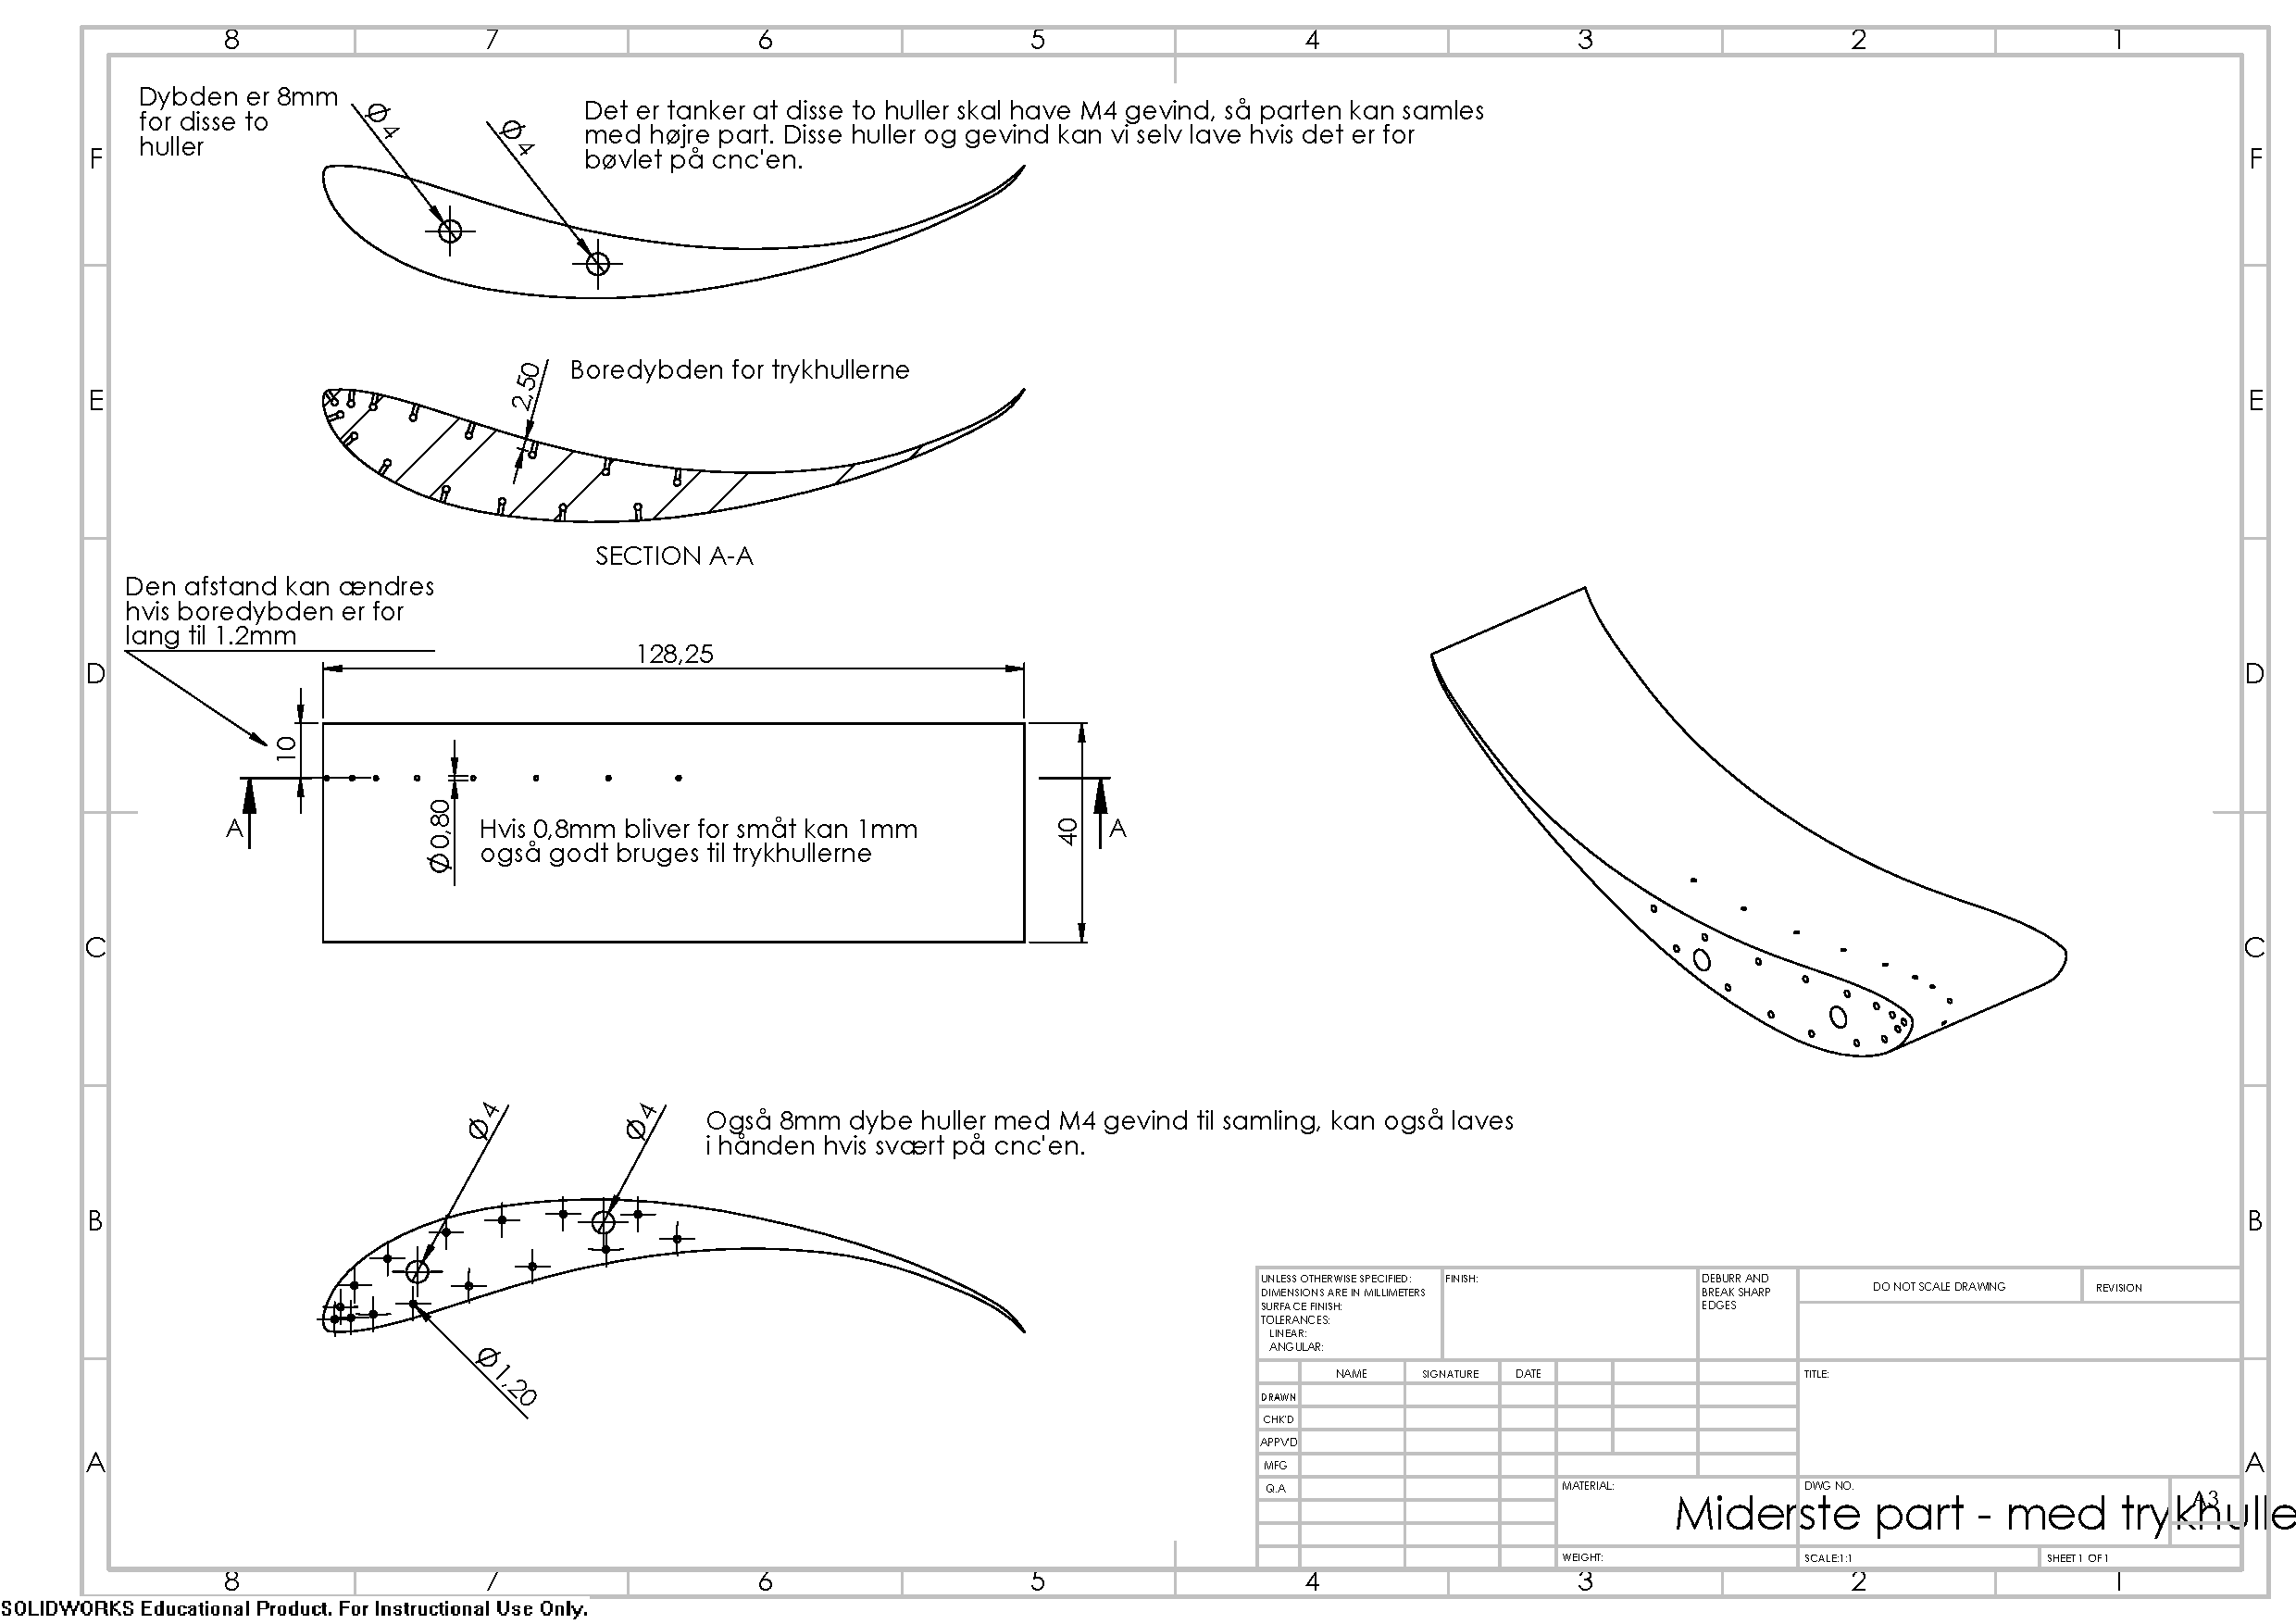
\includegraphics[width = \textwidth]{arbejdstegningvindtunnel}
      \caption{Blueprints of the centerpiece of the wing containing the pressure taps for generating a pressure distribution profile.}
      \label{fig:scalewingblueprint}
    \end{figure}

    \begin{figure}
      \begin{subfigure}[b]{\textwidth}
        \includegraphics[width=1\linewidth]{windtunnelright}
        \caption{Blueprints of the right section of the wing.}
        \label{fig:scalewingblueprintright}
      \end{subfigure}

      \begin{subfigure}[b]{\textwidth}
        \includegraphics[width=1\linewidth]{windtunnelleft}
        \caption{Blueprints of the left section of the wing with a pocket allowing pressure tubes to be fed through. Additionally fitted with an $\diameter \SI{8}{\milli\metre}$ H7 hole for mounting the wing vertically.}
        \label{fig:scalewingblueprintleft}
      \end{subfigure}
    \end{figure}

    \begin{figure}
      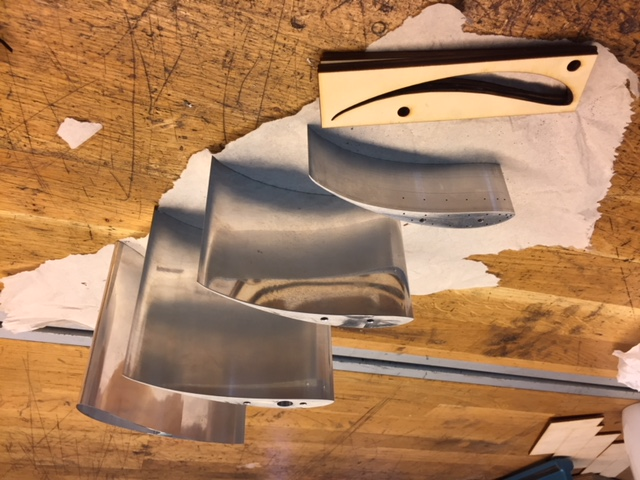
\includegraphics[width=\textwidth, rotate=180]{scalewing}
      \caption{Pieces of the downscaled wing before assembly. Additional H7 holes had to be drilled in order to mount the wing to the force gauge securely.}
      \label{fig:scalewingparts}
    \end{figure}

    After the initial analysis of airfoils, this design was chosen based on preliminary research. From \cite{winginitialangle}, a rule of thumb for multi element design is that the first element should be around $70\%$ of the total chord length, and the second element around $30\%$. From \cite{jkatz}, the initial position of the elements was chosen. Having the perfect position is not essential, as the experiment is a simply a verification method of the computational method, which will be used to optimize the final design.

    The 1/4 scale rear wing was machined at Philips Lighting by Rasmus Himborg based on the technical drawings presented in the following section.

    \subsubsection{Blueprints}

      The wing requires a series of small holes for the measurements needed. 15 holes have to be made along the very narrow wing profile to measure the pressure on the wing's surface. The pressure taps have to be $\diameter\SI{0.8}{\milli\metre}$ on the outside, with an inner bore hole with $\diameter\SI{1.2}{\milli\metre}$ to have a syringe inserted. The wing needs to be separated into smaller parts, as drilling $\diameter\SI{1.2}{\milli\metre}$ pressure inlets throughout the entire wing is very difficult. Thus, the large wing is dissected into three parts. A central part with 15 pressure taps, and two regular wings with holes for pressure tubes to escape. The left section contains a H7 hole for fitting the wing in the wind tunnel and leading the pressure tubes to the pressure transducer. The right wing is a basic wing with holes for mounting. These two parts can be seen in figures \ref{fig:scalewingblueprintright} and \ref{fig:scalewingblueprintleft}. Aligning the three wing sections has to be fairly accurate. The center wing thus carries threaded holes, and the adjacent wings has M4 holes where a threaded rod can align the wings securely. The final design of the centerpiece can be seen in figure \ref{fig:scalewingblueprint}.

      Material selection is based on the ease of machinability - a CNC-miller was provided to us, along with ample amounts of aluminium. This scale wing is not to be used in the actual race car, so weight is not a concern. Construction of the 1/4 scale wing is not trivial. High precision is required for the surface finish, and the pressure taps have to be small in diameter: $\diameter\SI{0.8}{\milli\metre}$ and very deep. This is not an ordinary task and requires specialized tooling.

      The manufactured model wing can be seen in \ref{fig:scalewingparts}, taken shortly after receiving the parts back from Rasmus Himborg. The width of the centerpiece is based around the fact that potential upstream interference from misalignment of the wing profile sections would not cause issues around the pressure taps. %Emmons box

      \textsc{3D-printed parts}

        Due to machining cost and production time, the second element was 3D-printed on A Zortrax M200 3D printer at DTU Skylab. The two 3d printed parts were glued together using instant glue.

      \textsc{Assembly}

      \begin{figure}
        \includegraphics[width=\textwidth]{scalewingAssembled3}
        \caption{Down-scaled wing assmembled with a zoom in on the pressure taps. The length of the entire wing is approximately $\SI{250}{\milli\metre}$ with a total chord length of $\SI{150}{\milli\metre}$.}
        \label{fig:scalewing}
      \end{figure}

      In figure \ref{fig:scalewing} the down-scaled wing post-production with pressure tubes inserted can be seen with pressure-taps along the centerpiece. The wing is assembled by lasercutting the two end plates with holes for mounting, as well as the H7 mounting hole and exits for the pressure tubes.

      In order to strengthen the construction and smoothen the surface, the 3D-printed rearwing was reinforced using red tape (as seen in figure \ref{fig:scalewing}), and is additionally supported by a wooden centerpiece holding the two wings together. Lastly, the small wing is reinforced further by attaching screws through the end plate, ensuring the wing does not flex.

\section{Experimental Procedure}

  The model wing's $\diameter\SI{8}{\milli\metre}$ hole is fitted with a rod at the end as seen to the left in figure \ref{fig:scalewing}, which is then mounted to the force gauge at the bottom of the wind tunnel. It is important the wing is placed as close to true level, in order to not get a skewed angle of attack initially \cite{truelevel}. The pressure measurement tubes are passed through a hole in the bottom of the wind tunnel's test section. Connection is established to the LabVIEW software running on a nearby computer. A picture of the data collection UI can be found in appendix \ref{app:labviewview}.

  The wing is positioned with a $0^\circ$ angle of attack. Measurements are taken with $\SI{10}{\metre\per\second}$ increments in the range of $\SIrange{10}{60}{\metre\per\second}$, with an angular sweep at $\SI{20}{\metre\per\second}$ and $\SI{40}{\metre\per\second}$ to compare the optimum angle of attack with literature.

  However, due to the wing covering a relatively large area of the wind tunnel, the final test could only go to $\SI{59.2}{\metre\per\second}$, which corresponds to $\SI{14.8}{\metre\per\second}$ or $\SI{53.3}{\kilo\metre\per\hour}$. Albeit slightly lower than optimimal, it is not far out of the proposed range.

\section{Results}

  The results from the experiment is divided into two parts: A comparison with the theoretical lift values of the downscaled wing, and a comparison with the simulated results. The simulated results will be shown in section \ref{sec:simulationcomparison}, while the comparison to theory can is shown below.

  \begin{figure}
    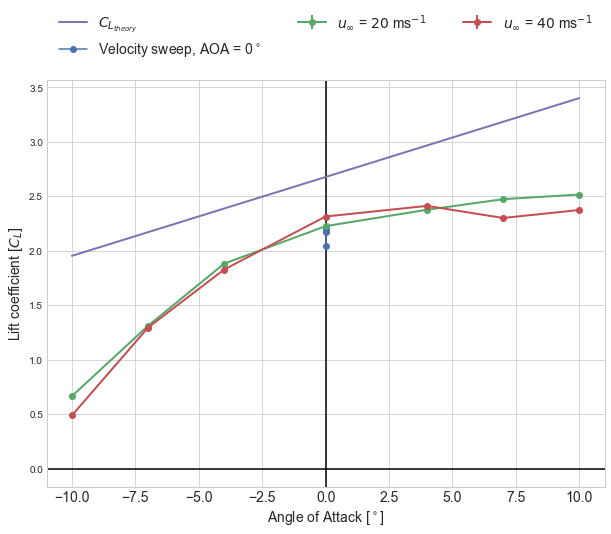
\includegraphics[width=\textwidth]{clperAOAexperiment}
    \caption{The lift coefficient plotted as a function of the wing's overall AOA. The wing's own angle of attack is $35^\circ$, which is beyond the theoretical optimum as seen in figure \ref{fig:AOAofairfoils}.}
    \label{fig:clperAOAexperiment}
  \end{figure}

  The theoretical lift coefficient at of the scale wing using a total AOA of $\alpha = 37^\circ$, an effective additional AOA from the wing's camber of $\alpha_{L_0} = 0^\circ$ and equation \ref{eq:CL} is found to be:
  \begin{align*}
    C_L &= \frac{C_{L0}}{1+\frac{C_{L0}}{\pi \AR}}
    \intertext{and remember that:}
    C_{L0} &= 2\pi (\alpha + \alpha_{L_0})\\
    \Rightarrow C_L &= \frac{2\pi \left(\frac{38\pi}{180}\right)}{1+\frac{2\pi \left(\frac{38\pi}{180}\right)}{\pi \frac{\SI{250}{\milli\metre}}{\SI{150}{\milli\metre}}\left(1+1.9\frac{\SI{175}{\milli\metre}}{\SI{250}{\milli\metre}}\right)}} = 3.1
  \end{align*}

  Comparing the theoretical lift to the lift coefficients found by the experiments is seen in figure \ref{fig:clperAOAexperiment}. The purple line is the theoretical lift, where the wing's angle is swept between $-10^\circ$ and $10^\circ$. The measured lift is slightly lower than the theoretical, which may be explained by the end plate's effect on aspect ratio. The downscaled wing has a very large $\AR$, where the end plates extend far below the bottom of the wing. While theoretically beneficial, the effect of the long end plates might not extend all the way up to the wing profile, artificially inflating up the theoretical lift number. Another effect is seen in figure \ref{fig:endplatesbending}, albeit a bit difficult to see, the end plates bend down due to the suction force. This might have reduced flow underneath the wing, constricting airflow and reducing the overall lift. The deflection was approximately $\SI{10}{\milli\metre}$ on each end plate.

  \begin{figure}
    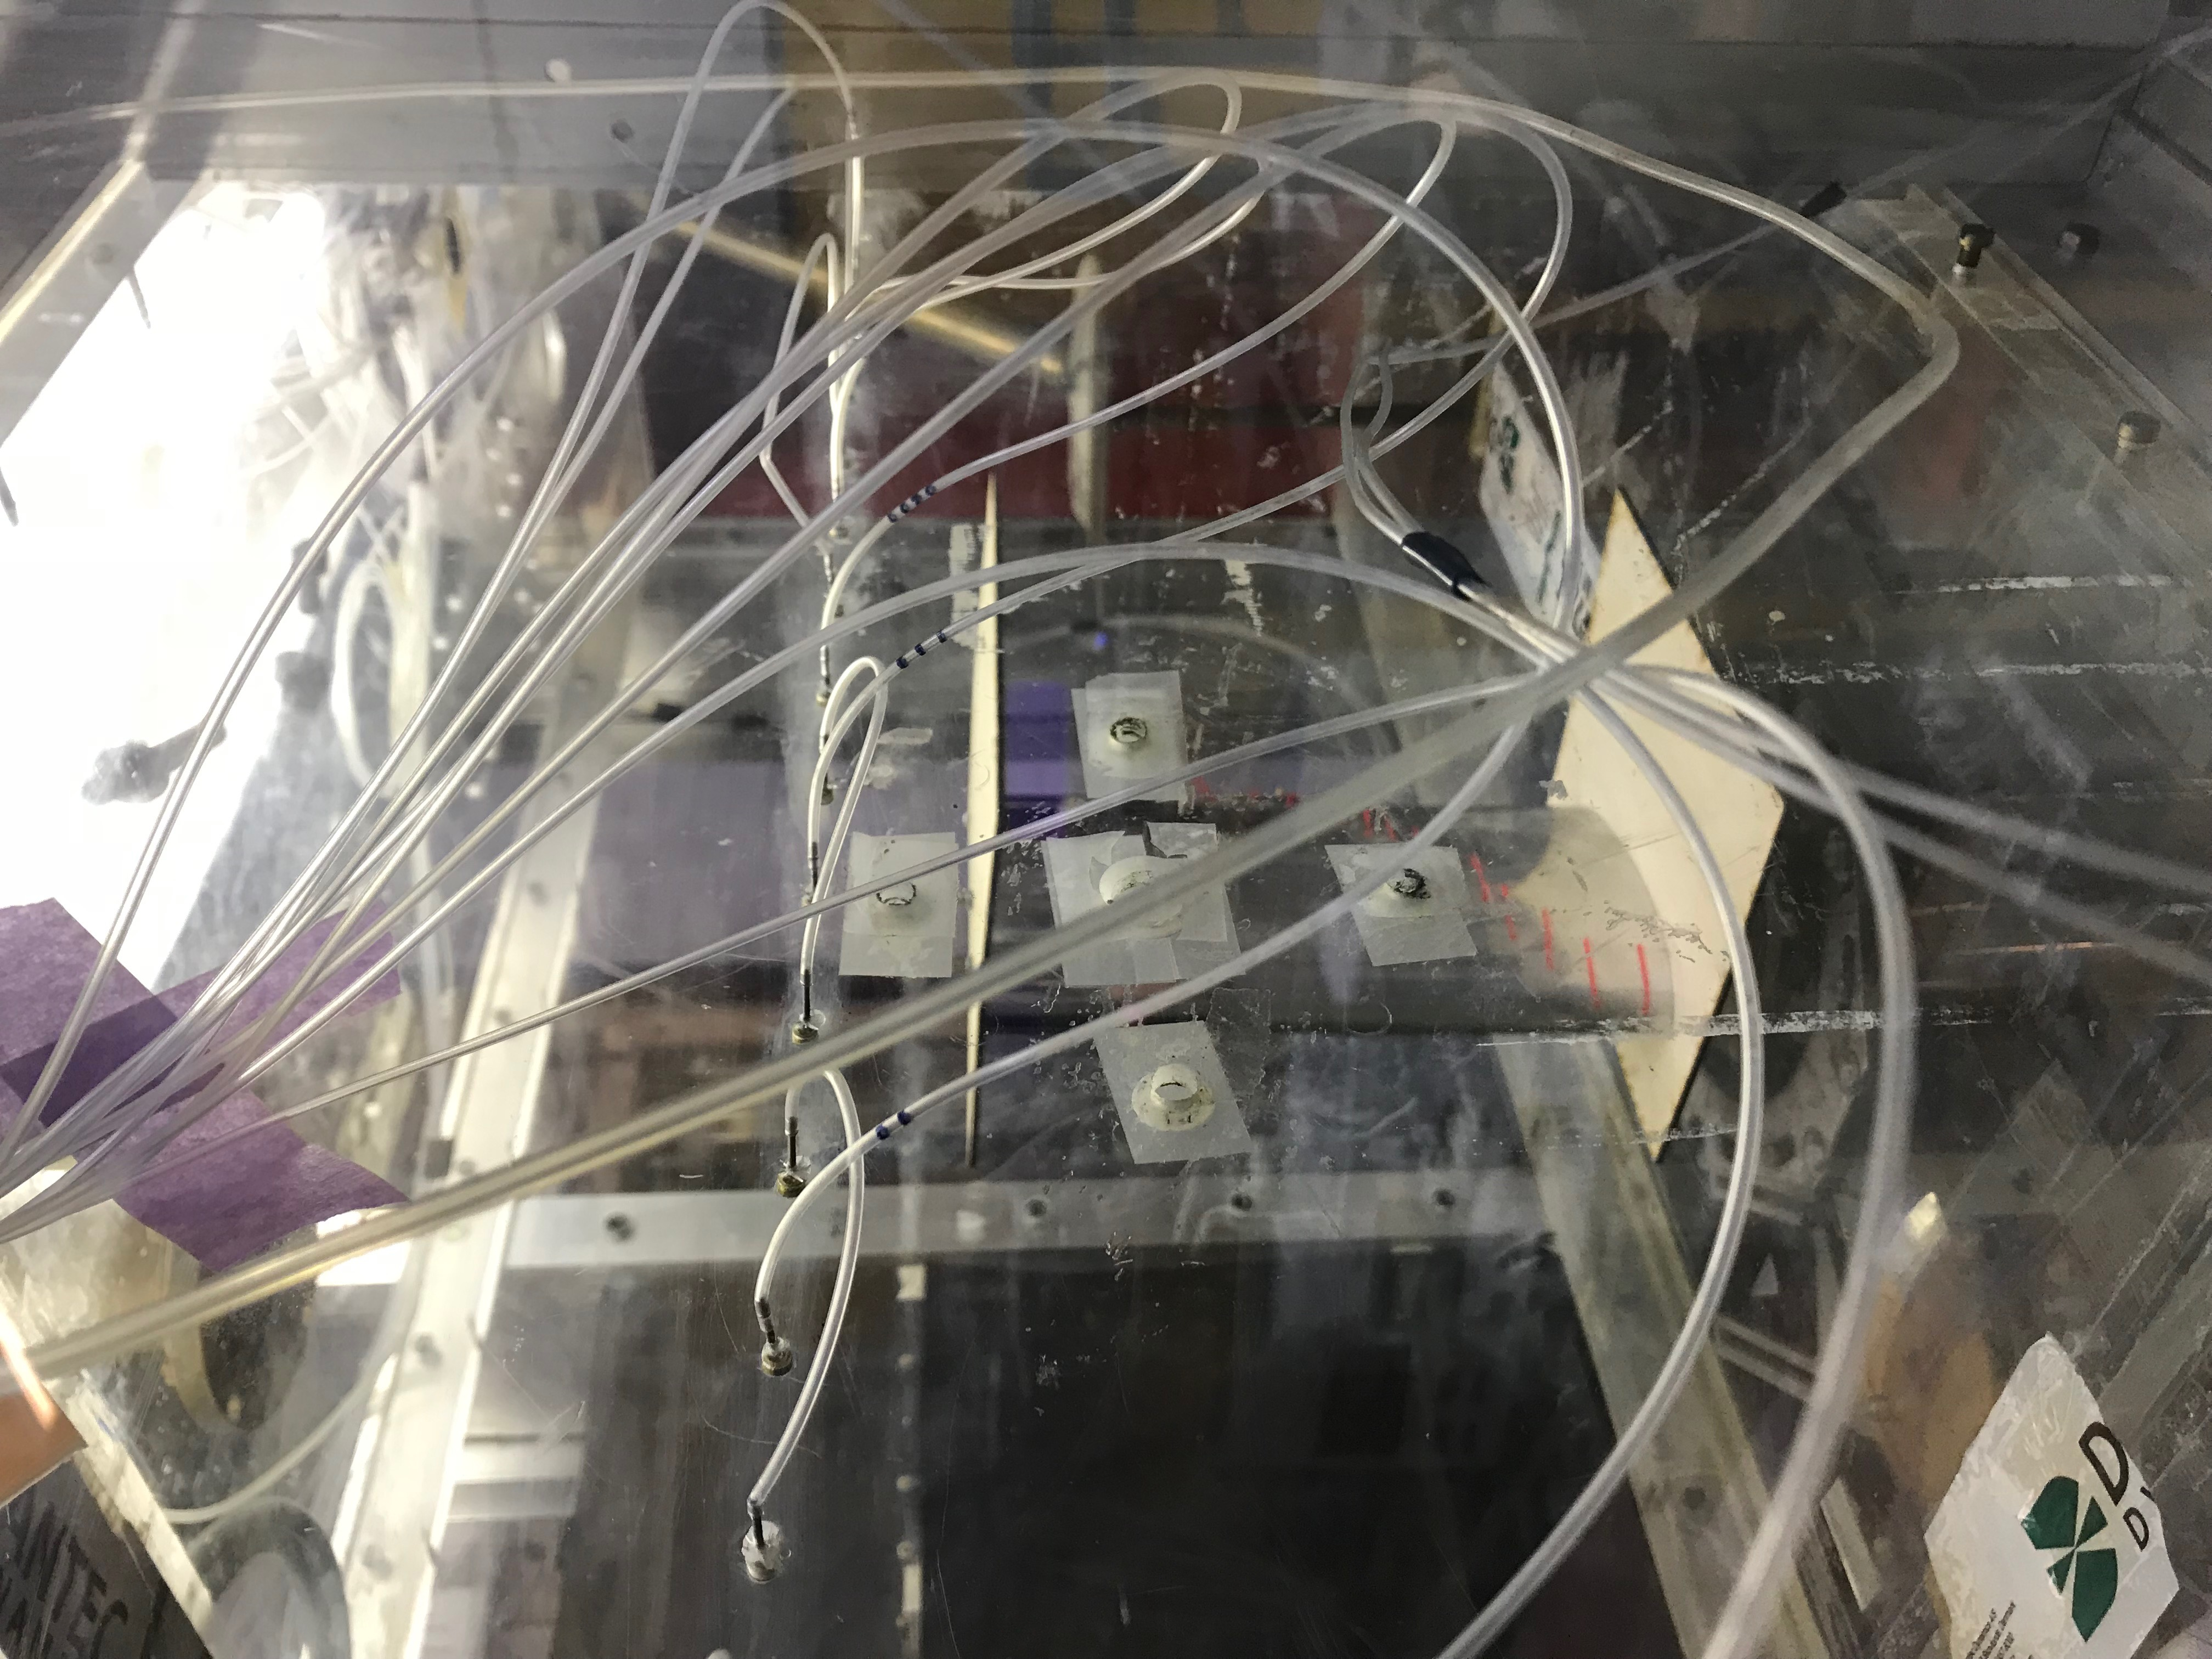
\includegraphics[width=\textwidth]{endplatesbending}
    \caption{The upper end plate can be seen deflecting slightly downward due to the suction force the wing exerts. }
    \label{fig:endplatesbending}
  \end{figure}
